\section{商品评论标签提取}
在了解了商品细节信息(如参数)之后,消费者通常也希望看到已买的人的评价,来作为自己是否要购买该商品的一个重要参考。于是乎,我们为了呈现这一部分信息,需要找到买家评价。但是,如下图\ref{img:yhb1}所示,评价部分并不是直接显示在网页源代码中的。

%插入图片
\begin{figure}[htbp]
\centering
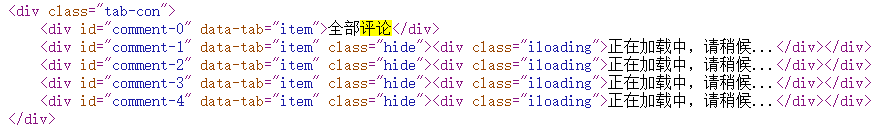
\includegraphics[width=13.5cm]{img/yhb/web_source_code_jd.png}
\caption{京东网页源码中查询评价的结果} %图片下方文字标签
\label{img:yhb1}   % 引用标记,用于文章中引用
\end{figure}

这也就是说,我们在之前爬到的HTML文件中是找不到评论信息的。
那么评论到底在哪里呢?简单想想,既然不在这个网址上,那么就一定在它会发送请求的某个网址上。下面不妨试一下,打开一个感兴趣的京东商品。我们在页面中鼠标右键选择检查(或F12)调出浏览器的调试窗口。然后点击network查看所有类型的请求(ALL),点击评论按钮使其加载数据。如下图\ref{img:yhb2}所示:

%插入图片
\begin{figure}[htbp]
\centering
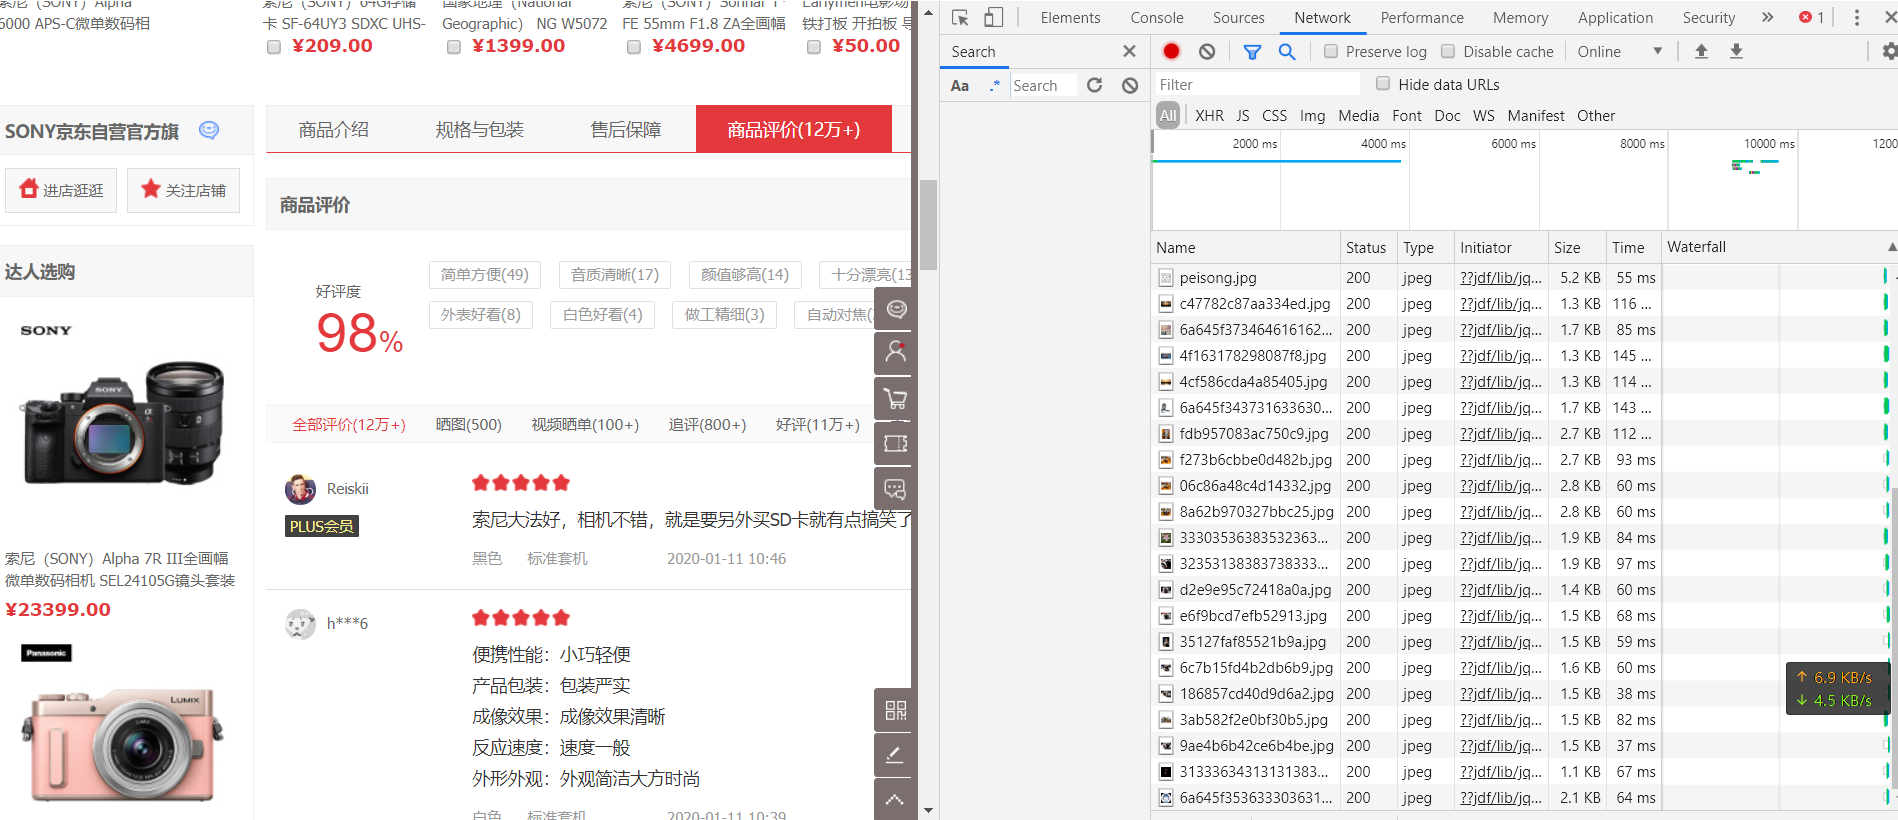
\includegraphics[width=13.5cm]{img/yhb/network_jd.png}
\caption{加载请求} %图片下方文字标签
\label{img:yhb2}   % 引用标记,用于文章中引用
\end{figure}

接着,查找加载评论数据的请求。我们可以使用某条评论中的一段话,然后在调试窗口中搜索。如下图\ref{img:yhb3}所示:
%插入图片
\begin{figure}[htbp]
\centering
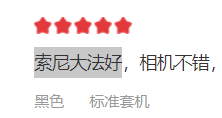
\includegraphics[width=13.5cm]{img/yhb/find_request_jd.png}
\caption{找到评论所在的请求} %图片下方文字标签
\label{img:yhb3}   % 引用标记,用于文章中引用
\end{figure}

搜索框下面返回的结果就是了。点击,在右面的headers里面可以看到request url,在preview里可以看到这个url里面的信息。如下图\ref{img:yhb4}:
%插入图片
\begin{figure}[htbp]
\centering
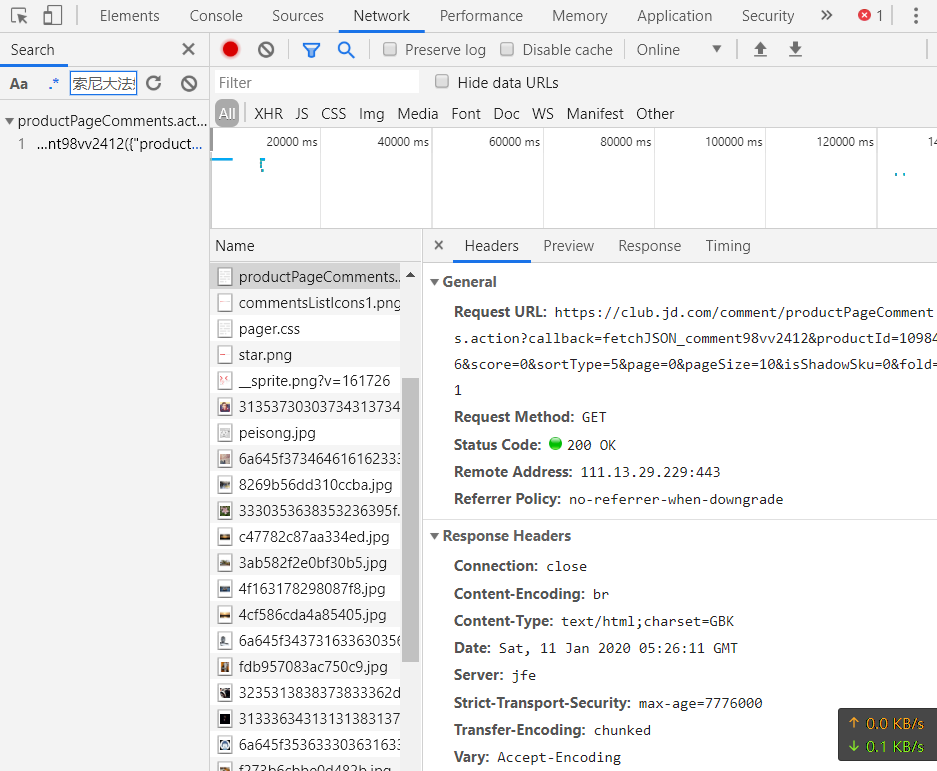
\includegraphics[width=13.5cm]{img/yhb/find_url_jd.png}
\caption{找到url} %图片下方文字标签
\label{img:yhb4}   % 引用标记,用于文章中引用
\end{figure}

在这个“fetchJSON\_comment”里面,有我们想要的评论信息。第一个标签comments,是评论的内容;第二个是评论的标签;第三个是评论的好评数量等数据统计。如下图\ref{img:yhb5}所示:
%插入图片
\begin{figure}[htbp]
\centering
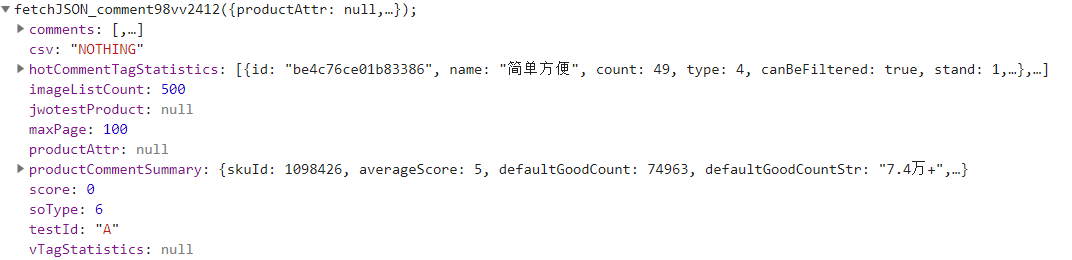
\includegraphics[width=13.5cm]{img/yhb/json_items_jd.png}
\label{img:yhb5}   % 引用标记,用于文章中引用
\end{figure}



一开始完成这个脚本的时候,设计的功能是将评论的内容(第一部分)爬下来。下图\ref{img:yhb6}展示了一些例子:
\begin{figure}[htbp]
\centering
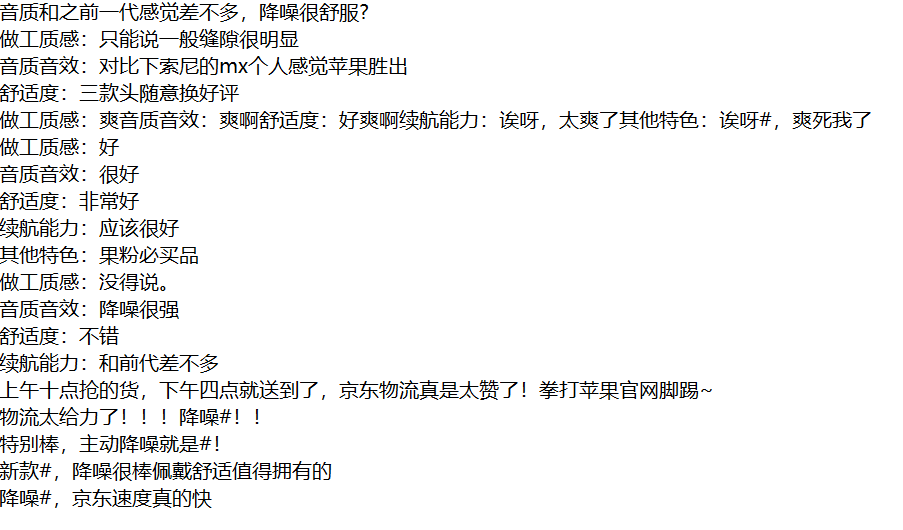
\includegraphics[width=13.5cm]{img/yhb/cmt_contents_eg_jd.png}
\caption{airpods pro的评论文字} %图片下方文字标签
\label{img:yhb6}   % 引用标记,用于文章中引用
\end{figure}
但这样做存在问题:一是,对于我一开始爬的上万个商品,将评论的文字全部弄下来空间占用太大了,建索引也会不方便;二是,我们想要实现的是商品的聚类检索,点击商品标签是可以直接跳到原商品网页的,不能,也没有必要在搜索结果上显示评论。因此,我希望通过商品的\textbf{评论标签}来对商品的特性进行说明。并通过\textbf{打分}来给商品一个基本的评定。

在明确了任务,并找到了接口之后,我们就可以开始写代码抓取数据了。一般我们会先尝试抓取一条数据,成功之后,我们再去分析如何实现大量抓取。下面的代码是在Windows环境下的python3里实现的。

\subsection{爬取评论数据}
经过上面的寻找和分析,可以确定url具有下面的格式:
%插入代码
\begin{python}
url=r"https://sclub.jd.com/comment/" \
    r"productPageComments.action?callback=fetchJSON_comment98vv106813&" \
    r"productId={}&" \
    r"score=0&sortType=5&page=0&pageSize=10&isShadowSku=0&fold=1".format(prdtId)
comment_tag_path = r'C:\TC-prog\JetBrain_pycharm_TC' \
                   r'\PycharmProjects\Crawler_EEFinal' \
                   r'\jd_cmt_tags\httpsitem.jd.com{}.html.txt'.format(prdtId)
try:
    r=requests.get(url,headers=headers,timeout=5)
    r.raise_for_status()
except:
    print ('爬取失败')
\end{python}
通常,我们会对爬虫脚本进行伪装,使之看起来更像是浏览器。下面设置请求中头文件的信息:
%插入代码
\begin{python}
headers = {'User-Agent':'Mozilla/5.0 '
                        '(Windows NT 10.0; Win64; x64) '
                        'AppleWebKit/537.36 (KHTML,'
                        ' like Gecko) Chrome/76.0.3809.132 '
                        'Safari/537.36',
#'Accept':'text/html;q=0.9,*/*;q=0.8',
#'Accept-Charset':'ISO-8859-1,utf-8;q=0.7,*;q=0.3',
#"Accept-Language": "zh-CN,zh;q=0.9",
#'Connection':'close',
'Referer':'https://www.jd.com/'
}
\end{python}
如果没有这个请求头,request返回的内容很有可能为空。

\subsection{提取数据}
我们对爬取的数据分析发现,此数据为jsonp跨域请求返回的json结果,所以我们只要把前面的\textbf{fetchJSON_comment98vv4646(}和最后的\textbf{)}去掉就拿到json数据了。

\begin{python}
raw = r.text[:]
pos = 0#这样写可以裁掉不一样长的前面这一串
for i in range(len(raw)):
    if raw[i] == '(':
        pos = i
try:
    r_json_str = r.text[pos + 1:-2]
    # print (r_json_str)
    r_json_obj=json.loads(r_json_str,strict=False)
    print (r_json_obj)
    r_json_tags=r_json_obj['hotCommentTagStatistics']
    print ('评论标签:')
\end{python}
上面的代码需要调用json库,json.loads函数将json对象转化成python的内置类型,在这里是字典。后面就按python dict类型进行操作了。
由下图\ref{img:yhb7}可以看见:每一个标签名都是在name字段下的,对应的数目是count。
%插入图片
\begin{figure}[htbp]
\centering
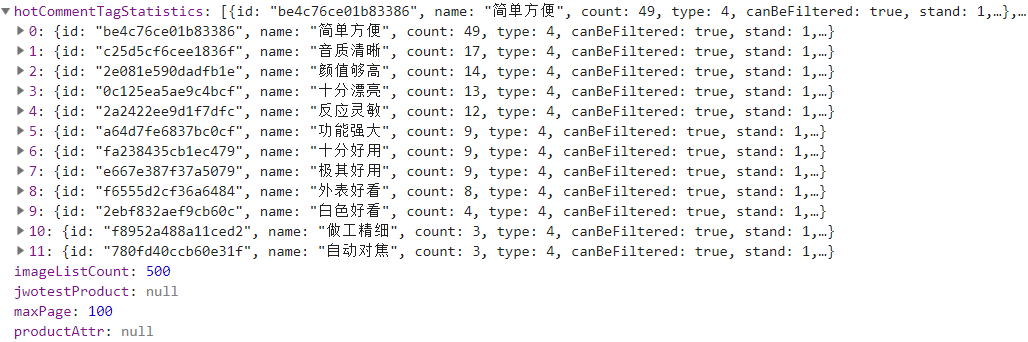
\includegraphics[width=13.5cm]{img/yhb/cmt_tags_eg_jd.png}
\label{img:yhb7}   % 引用标记,用于文章中引用
\end{figure}
可以根据这点读取评论的标签和数量:
\begin{python}
print(r_json_tag['name']+
                      '\t'+str(r_json_tag['count']))
\end{python}
\subsection{写入文件}
数据提取后我们需要将他们保存起来,一般保存数据的格式主要有:文件、数据库、内存这三大类。今天我们就将数据保存为txt文件格式,因为操作文件相对简单同时也能满足我们的后续数据分析的需求:
\begin{python}
# 追加模式,逐行写入

        for r_json_tag in r_json_tags:
            with open(comment_tag_path,'a+') as file:
                file.write(r_json_tag['name']+
                           '\t'+str(r_json_tag['count'])+'\n')
                print(r_json_tag['name']+
                      '\t'+str(r_json_tag['count']))
\end{python}
NOTE: 由于后面进行批量爬取的时候很有可能出现爬取失败的情况,上面的内容要放进try\&except里。

\subsection{批量爬取及多线程}
由于要处理的对象数目庞大,仅仅使用线性的程序不只是慢,而且可靠性也会大打折扣。所以这个脚本需要写成多线程的,来保证程序不会因为一个线程的终止而停下来。从我实现的顺序,是先完成了重复爬取,再写的多线程,现在不妨就一起介绍了。

注意到请求的url具有相对稳定的格式,仅有两处是变化的:一是“fetchJSON\_comment98vv106813”这样的一串,二是后面的商品ID(通过商品页url可以过滤出来)。经过多次实验,可以发现对于第一串,只要具有形如fetchJSON\_comment98vv106813的格式,请求往往都是可以被接受的。于是在封装的函数里,比较容易写出一般形式的url:
\begin{python}
url=r"https://sclub.jd.com/comment/" \
        r"productPageComments.action?callback=fetchJSON_comment98vv106813&" \
        r"productId={}&" \
        r"score=0&sortType=5&page=0&pageSize=10&isShadowSku=0&fold=1".format(prdtId)
\end{python}
将前面的步骤封装进函数:
\begin{python}
def crawl_jd_cmt_tag(prdtId):# change for url

    url=r"https://sclub.jd.com/comment/" \
   	   r"productPageComments.action?callback=fetchJSON_comment98vv106813&" \
 	   r"productId={}&" \
 	   r"score=0&sortType=5&page=0&pageSize=10&isShadowSku=0&fold=1".format(prdtId)
    comment_tag_path = r'C:\TC-prog\JetBrain_pycharm_TC' \
                   r'\PycharmProjects\Crawler_EEFinal' \
                   r'\jd_cmt_tags\httpsitem.jd.com{}.html.txt'.format(prdtId)

    try:
        r=requests.get(url,headers=headers,timeout=5)
        r.raise_for_status()
    except:
        print ('爬取失败')

    raw = r.text[:]
    pos = 0
    for i in range(len(raw)):
        if raw[i] == '(':
            pos = i
    try:
        r_json_str = r.text[pos + 1:-2]
        r_json_obj=json.loads(r_json_str,strict=False)
        r_json_tags=r_json_obj['hotCommentTagStatistics']
        
        # 追加模式,逐行写入

        for r_json_tag in r_json_tags:
            with open(comment_tag_path,'a+') as file:
                file.write(r_json_tag['name']+
                           '\t'+str(r_json_tag['count'])+'\n')
                print(r_json_tag['name']+
                      '\t'+str(r_json_tag['count']))
    except:
        print('failed')
\end{python}

接下来设置多线程,执行上述函数:
\begin{python}
q = queue.Queue()
NUM = 5
JOBS = 10

def run():
    global f
    for line in f.readlines():
        try:
            pp = line.split('\t')
            webpage = pp[1].strip('\n')
            print(webpage)
            temp = webpage[14:-5]
            pos = 0
            for i in range(len(temp)):
                if temp[i] == 'm':
                    pos = i
            itemID = temp[pos + 1:]
            print(itemID)
            if (len(webpage) > 35):
                continue
            print(itemID)
            crawl_jd_cmt_tag(itemID)
            time.sleep(random.random() * 3)
        except:
            print("Invalid Input!")

def working():
    while True:
        #arguments = q.get()
        run()
        q.task_done()


#fork NUM个线程等待队列
for i in range(NUM):
    t = Thread(target=working)
    t.setDaemon(True)
    t.start()
#把JOBS排入队列
for i in range(JOBS):
    q.put(i)
#阻塞,等待所有JOBS完成
q.join()
f.close()
\end{python}
NOTE:有必要解释一下run函数中的工作。爬取2w+条商品生成了一个记录了这些商品的url的表格(.txt)。而这些url中含有对应每个商品的ID。run函数的工作就是抽出ID,调用专用于评论的爬虫函数,来记录评论标签。

运行结果\ref{img:yhb8}\ref{img:yhb9}:
%插入图片
\begin{figure}[htbp]
\centering
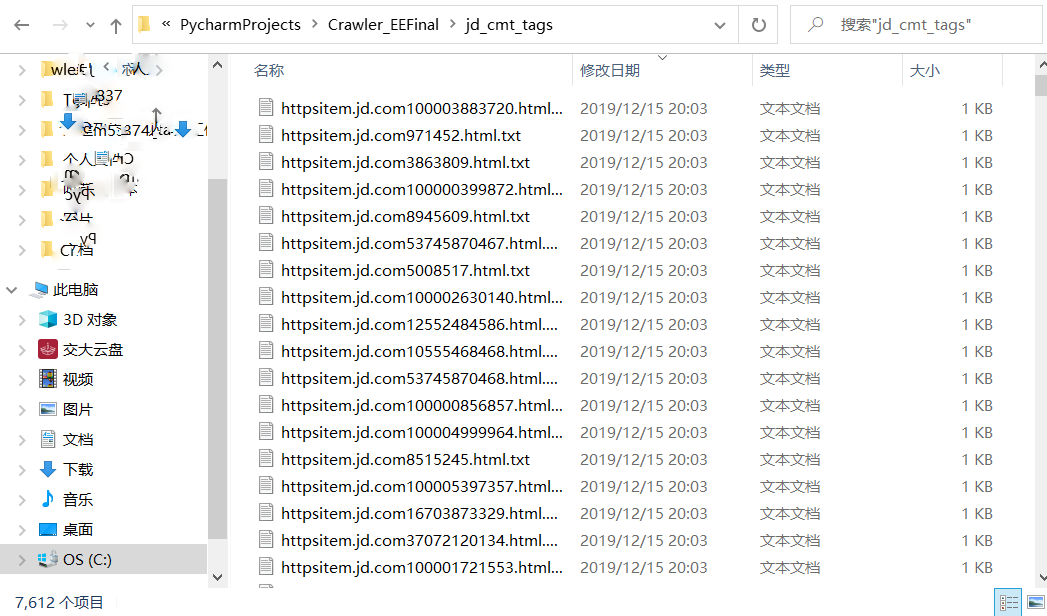
\includegraphics[width=13.5cm]{img/yhb/folder_view_jd.png}
\caption{文件夹中显示,已打码处理} %图片下方文字标签
\label{img:yhb8}   % 引用标记,用于文章中引用
\end{figure}
\begin{figure}[htbp]
\centering
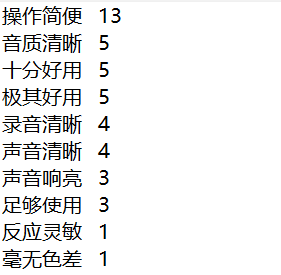
\includegraphics[width=13.5cm]{img/yhb/contents_eg_jd.png}
\label{img:yhb9}   % 引用标记,用于文章中引用
\end{figure}

这一部分工作就完成了。下面,将按相似的流程完成商品的评分。



\section{商品评分计算}
程序的工作流程和整体框架和爬取标签时的一样,但需要更改存储路径和对json对象信息的处理方式。具体来说,需要抽取不同属性的数据,并设计一个评估商品优劣的数值算法。preview该请求\ref{img:yhb10},看一下productCommentSummary里的内容:

\begin{figure}[htbp]
\centering
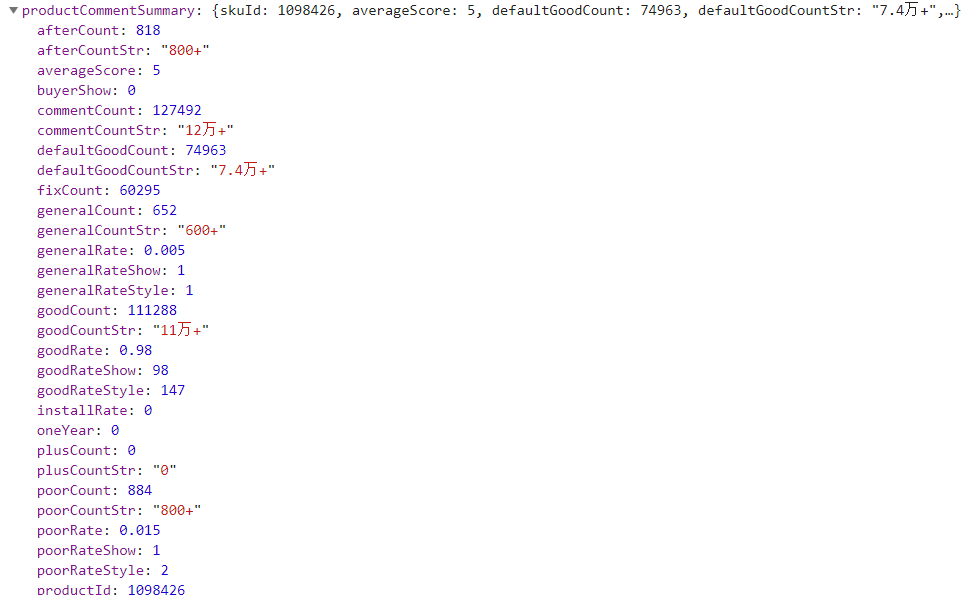
\includegraphics[width=13.5cm]{img/yhb/data_eg_jd.png}
\caption{productCommentSummary内容的部分截图}
\label{img:yhb10}  % 引用标记,用于文章中引用
\end{figure}

在这些数据里,好评率可以反映消费者的满意程度,评论总数可以反映商品销量和热度,追评和视频评价则可以一定程度体现消费者对商品的重视程度。将这些信息综合考虑,可以设计下面计算商品分数的公式:

\begin{python}
score=int(rate*0.7+math.log10(sumcmt)*5+
                          ((after+video)*1.0)/sumcmt/0.05)
\end{python}

实现打分的代码块如下:
\begin{python}
    try:
        r_json_str = r.text[pos + 1:-2]
        r_json_obj=json.loads(r_json_str,strict=False)
        r_json_Sum=r_json_obj['productCommentSummary']
        # 追加模式,逐行写入
        with open(comment_tag_path, 'w') as file:
            sumcmt=r_json_Sum['commentCount']
            rate=r_json_Sum['goodRateShow'] # 好评率*100
            video =r_json_Sum['videoCount']
            after =r_json_Sum['afterCount']

            score=int(rate*0.7+math.log10(sumcmt)*5+
                          ((after+video)*1.0)/sumcmt/0.05)


            file.write("httpitem.jd.com"+str(prdtId) +".html"
                       + '\t' + str(score) + '\n')
            print("httpsitem.jd.com"+str(prdtId) +".html"
                       + '\t' + str(score))

    except:
        print('failed')
\end{python}

运行结果\ref{img:yhb11}:
\begin{figure}[htbp]
\centering
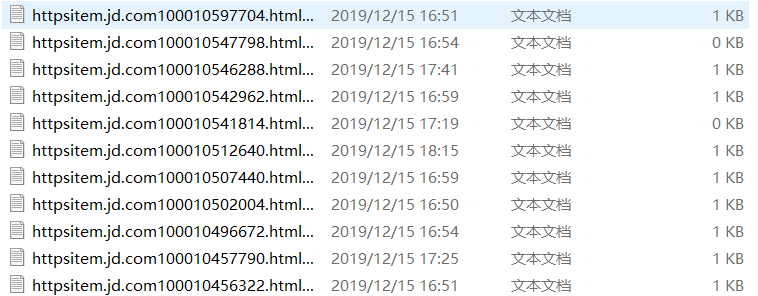
\includegraphics[width=13.5cm]{img/yhb/res1_jd.png}
\caption{在文件夹中显示}
\label{img:yhb11}   % 引用标记,用于文章中引用
\end{figure}
\ref{img:yhb12}
\begin{figure}[htbp]
\centering
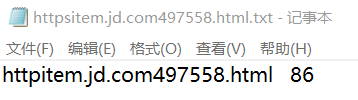
\includegraphics[width=13.5cm]{img/yhb/res2_jd.png}
\caption{内容示例}
\label{img:yhb12}   % 引用标记,用于文章中引用
\end{figure}


\subsection{遇到的问题及其解决}
在运行较早版本的评论爬虫的时候,有时会像下面这样\ref{img:yhb13}:
\begin{figure}[htbp]
\centering
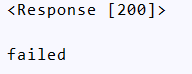
\includegraphics[width=13.5cm]{img/yhb/error_eg.png}
\caption{错误示例}
\label{img:yhb13}   % 引用标记,用于文章中引用
\end{figure}
为什么会变成这样呢?
稍加修改脚本可以使之强制创建文件(当然没法写入内容),可以看到\ref{img:yhb14}这样的结果:
\begin{figure}[htbp]
\centering
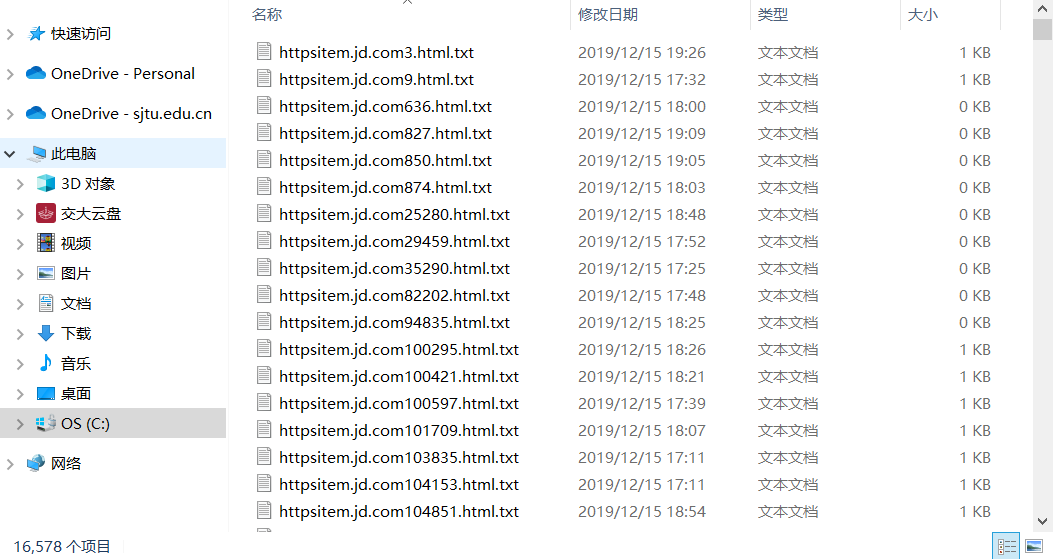
\includegraphics[width=13.5cm]{img/yhb/files_jd.png}
\caption{在文件夹中显示}
\label{img:yhb14}  % 引用标记,用于文章中引用
\end{figure}
可以看到,不少商品的ID变为了十位,甚至个位数——这在京东上是无法找到对应商品的。而ID参数是由int类型传递的。\ref{img:yhb15}
\begin{figure}[htbp]
\centering
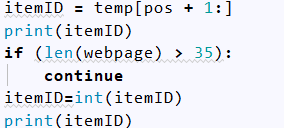
\includegraphics[width=13.5cm]{img/yhb/problem_code.png}
\label{img:yhb15}
\end{figure}
可以推测,是转为int时前面的0消失了。删去类型转换,以字符串传参,问题解决。

到这里,我们就完成了京东的评论标签爬取和分数评定。后面我还将介绍苏宁商品的这些操作。















